% =====================================================================
% Group 4 -- Meta-Analysis Seminar (Prof. Rainer Winkelmann, UZH, HS 2026)
% Report: Ethnic discrimination in hiring -- replication and update of
%         Zschirnt & Ruedin (2016)
%
% Location in the repo: 04_report/main.tex
% Tables and figures come from the Python code (02_code/run_all.py):
%   04_report/tables/*.tex   04_report/figures/*.pdf
% Every number in the text should come from a macro (\maORre etc.),
% never typed by hand.
% =====================================================================
\documentclass[11pt,a4paper]{article}

% ---------- packages ----------
\usepackage[utf8]{inputenc}
\usepackage[T1]{fontenc}
\usepackage{lmodern}
\usepackage[margin=2.5cm]{geometry}
\usepackage{setspace}
\onehalfspacing
\usepackage{amsmath,amssymb}
\usepackage{booktabs,longtable,array}
\usepackage{graphicx}
\usepackage{caption}
\usepackage[authoryear,round]{natbib}
\usepackage[hidelinks]{hyperref}

% ---------- numbers from the code ----------
% generated by 02_code/02_replication.py -- do not edit by hand
\newcommand{\maK}{34}
\newcommand{\maKsub}{215}
\newcommand{\maORfe}{0.63}
\newcommand{\maCIfe}{[0.61; 0.65]}
\newcommand{\maORuwls}{0.63}
\newcommand{\maCIuwls}{[0.56; 0.71]}
\newcommand{\maORre}{0.60}
\newcommand{\maCIre}{[0.52; 0.69]}
\newcommand{\maLnORre}{-0.509}
\newcommand{\maSEre}{0.070}
\newcommand{\maPIre}{[0.28; 1.27]}
\newcommand{\maTauSqRe}{0.141}
\newcommand{\maIsqRe}{92.7}
\newcommand{\maQ}{327.7}
\newcommand{\maIsqQ}{89.9}
\newcommand{\maORreKH}{0.60}
\newcommand{\maCIreKH}{[0.52; 0.70]}
\newcommand{\maORreDL}{0.61}
\newcommand{\maORrePM}{0.60}
\newcommand{\maORreNoBendick}{0.58}
\newcommand{\maCIreNoBendick}{[0.52; 0.65]}
\newcommand{\maORsub}{0.55}
\newcommand{\maCIsub}{[0.52; 0.58]}
\newcommand{\maSEratioUWLS}{3.15}
\newcommand{\maPctLowerOdds}{40}

% generated by 02_code/04_power_bias.py -- do not edit by hand
\newcommand{\maMedPower}{0.97}
\newcommand{\maMeanPower}{0.83}
\newcommand{\maNadequate}{24}
\newcommand{\maORwaap}{0.64}
\newcommand{\maCIwaap}{[0.55; 0.73]}
\newcommand{\maORpet}{0.69}
\newcommand{\maCIpet}{[0.53; 0.91]}
\newcommand{\maORpeese}{0.65}
\newcommand{\maFAT}{-1.05}
\newcommand{\maFATse}{1.29}
\newcommand{\maFATt}{-0.81}
\newcommand{\maShareSig}{0.79}
\newcommand{\maNsig}{27}
\newcommand{\maExpSig}{0.83}
\newcommand{\maESS}{-0.03}
\newcommand{\maExpSigTau}{0.70}
\newcommand{\maESSTau}{+0.10}
\newcommand{\maMedPowerNoBendick}{0.99}
\newcommand{\maMeanPowerNoBendick}{0.84}
\newcommand{\maNadequateNoBendick}{24}
\newcommand{\maORwaapNoBendick}{0.62}
\newcommand{\maCIwaapNoBendick}{[0.55; 0.70]}
\newcommand{\maORpetNoBendick}{0.72}
\newcommand{\maCIpetNoBendick}{[0.57; 0.90]}
\newcommand{\maORpeeseNoBendick}{0.64}
\newcommand{\maFATNoBendick}{-1.61}
\newcommand{\maFATseNoBendick}{1.09}
\newcommand{\maFATtNoBendick}{-1.48}
\newcommand{\maShareSigNoBendick}{0.79}
\newcommand{\maNsigNoBendick}{26}
\newcommand{\maExpSigNoBendick}{0.84}
\newcommand{\maESSNoBendick}{-0.05}
\newcommand{\maExpSigTauNoBendick}{0.73}
\newcommand{\maESSTauNoBendick}{+0.06}
\newcommand{\maMedPowerComb}{0.82}
\newcommand{\maMeanPowerComb}{0.68}
\newcommand{\maNadequateComb}{19}
\newcommand{\maORwaapComb}{0.76}
\newcommand{\maCIwaapComb}{[0.67; 0.85]}
\newcommand{\maORpetComb}{0.87}
\newcommand{\maCIpetComb}{[0.77; 0.99]}
\newcommand{\maORpeeseComb}{0.77}
\newcommand{\maFATComb}{-3.16}
\newcommand{\maFATseComb}{0.86}
\newcommand{\maFATtComb}{-3.67}
\newcommand{\maShareSigComb}{0.82}
\newcommand{\maNsigComb}{31}
\newcommand{\maExpSigComb}{0.68}
\newcommand{\maESSComb}{+0.14}
\newcommand{\maExpSigTauComb}{0.62}
\newcommand{\maESSTauComb}{+0.19}
\newcommand{\maORuwlsComb}{0.74}
\newcommand{\maORkline}{0.89}
\newcommand{\maNkline}{83'643}
\newcommand{\maWshareKline}{50}
\newcommand{\maWshareKlineRE}{3}
\newcommand{\maWshareOrig}{41}
\newcommand{\maKnoKline}{37}
\newcommand{\maORuwlsNoKline}{0.62}
\newcommand{\maMeanPowerNoKline}{0.85}
\newcommand{\maMedPowerNoKline}{0.99}
\newcommand{\maNadequateNoKline}{28}
\newcommand{\maMeanPowerCombRE}{0.86}
\newcommand{\maMedPowerCombRE}{1.00}
\newcommand{\maNadequateCombRE}{30}

% exists only after the update has been run with new studies:
\IfFileExists{tables/macros_update.tex}{% generated by 02_code/03_update.py -- do not edit by hand
\newcommand{\maKnew}{4}
\newcommand{\maKcomb}{38}
\newcommand{\maORcomb}{0.61}
\newcommand{\maCIcomb}{[0.54; 0.69]}
\newcommand{\maORnewMin}{0.47}
\newcommand{\maORnewMax}{0.89}
\newcommand{\maNnewInCI}{0}
}{}

% ---------- title page ----------
\title{Ethnic Discrimination in Hiring:\\
  A Replication and Update of Zschirnt and Ruedin (2016)}
\author{Kevin de Silva \and Vanessa Allenspach\\[1em]
  \small Group 4 -- MA Seminar ``Meta-Analysis'', Prof.\ Rainer Winkelmann\\
  \small University of Zurich, Fall 2026}
\date{13 November 2026}

\begin{document}

\begin{titlepage}
  \maketitle
  \thispagestyle{empty}
\end{titlepage}

\tableofcontents
\newpage

% =====================================================================
\section{Introduction}
% Vanessa -- ca. 1 page. DRAFT: rewrite in your own words.
% =====================================================================

Do job applicants with a foreign-sounding name get fewer invitations to a
job interview than equally qualified applicants from the majority population?
Unequal access to jobs is one of the most direct channels through which
ethnic inequality can arise and persist in the labour market. Because
employers rarely state discriminatory motives openly, it cannot be measured
by simply asking them.

Field experiments known as \emph{correspondence tests} address this problem.
Researchers send fictitious but otherwise identical applications to real job
vacancies and vary only the signal of ethnicity, usually the applicant's
name. The difference in positive responses (\emph{callbacks}) between
minority and majority applicants then measures discrimination at the first
stage of hiring.

Since 1990, dozens of such experiments have been conducted in many countries.
\citet{zschirnt2016} combine them in a meta-analysis of \maK{} studies and
find that minority applicants have substantially lower odds of a callback
(odds ratio \maORre{} \maCIre).

In this report we (i)~replicate the pooled estimate of \citet{zschirnt2016}
with fixed-effect (FE), random-effects (RE) and unrestricted weighted least
squares (UWLS) estimators, (ii)~update the meta-analysis with
\IfFileExists{tables/macros_update.tex}{\maKnew}{four} more recent studies,
(iii)~assess the statistical power of the literature, and (iv)~examine the
evidence for publication bias. We conclude by asking whether the literature
provides reliable evidence on the true size of ethnic discrimination in
hiring.

% =====================================================================
\section{Research question and literature}
% Vanessa -- ca. 1.5 pages (task 1: X, outcome, design, equation, dataset)
% =====================================================================

\paragraph{Treatment and outcome.}
The treatment $X$ is the ethnic signal on an application: a name associated
with an ethnic minority instead of a name associated with the majority
population. The outcome $Y$ is a binary indicator for a positive employer
response (a callback), usually an invitation to a job interview or a request
for more information.

\paragraph{Design.}
In a correspondence test, researchers construct matched pairs (or sets) of
written applications that are equivalent in education, work experience and
other productive characteristics. The applications are sent to the same or
comparable vacancies, and the minority signal is randomly assigned. Random
assignment means that differences in callbacks can be attributed to the
ethnic signal rather than to differences in qualifications.

\paragraph{Typical estimating equation.}
Individual studies usually estimate a linear probability model
\begin{equation}
  \text{Callback}_{ij} = \alpha + \beta\,\text{Minority}_i
    + \gamma' X_{ij} + \varepsilon_{ij},
\end{equation}
where $\text{Callback}_{ij}$ indicates a positive response to application
$i$ for vacancy $j$, $\text{Minority}_i$ is the treatment indicator and
$X_{ij}$ contains control variables (for example occupation, region or
applicant characteristics). The coefficient $\beta$ is the difference in
callback rates between minority and majority applicants.

\paragraph{Typical dataset.}
A well-known example is \citet{bertrand2004}, who sent about 5{,}000
fictitious r\'esum\'es with distinctively white or African-American names to
job advertisements in Boston and Chicago.
% TODO: 2-3 sentences on what they found (check the paper).

\paragraph{Effect size used in the meta-analysis.}
Following \citet{zschirnt2016}, we summarise each study by the odds ratio
of a callback. With $a$ and $b$ the numbers of minority applications with
and without a callback, and $c$ and $d$ the same for the majority,
\begin{equation}
  OR_i = \frac{a_i / b_i}{c_i / d_i}, \qquad
  y_i = \ln OR_i, \qquad
  SE_i = \sqrt{\frac{1}{a_i} + \frac{1}{b_i} + \frac{1}{c_i} + \frac{1}{d_i}}.
\end{equation}
An odds ratio of one means no discrimination; values below one mean that
minority applicants are less likely to receive a callback.

% =====================================================================
\section{The original meta-analysis and data}
% Vanessa -- ca. 1.5 pages
% =====================================================================

\citet{zschirnt2016} collect correspondence tests on ethnic discrimination
in hiring in OECD countries conducted between 1990 and 2015. Their
replication data (Harvard Dataverse) contain 43 studies with 738 subgroup
comparisons. Only \maK{} of these studies, with \maKsub{} subgroups, report
the four callback counts needed to compute an odds ratio; these form the
basis of the pooled estimate.

Using a random-effects model, the authors find a pooled odds ratio of
\maORre{} \maCIre. In other words, minority applicants have about
\maPctLowerOdds{}\,\% lower odds of a callback than equally qualified
majority applicants.
% TODO: 1-2 sentences on their moderator results (region, skill level,
%       EU directives) -- check pp. 6-10 of the paper.

We use the authors' replication data without changes. The studies cover
North America, Australia and many European countries; the evidence table in
Appendix~\ref{app:evidence} lists all studies with their effect sizes.

% =====================================================================
\section{Replication}
% both -- task 2: FE, RE, UWLS; which CI is wider and why
% =====================================================================

\begin{table}[htbp]
\centering
\small
\caption{Replication of the pooled effect (study level, $k = 34$)}
\label{tab:replication}
\begin{tabular}{lrrrrrrr}
\toprule
Method & $k$ & $\ln OR$ & SE & OR & 95\% CI (OR) & $\hat\tau^2$ & $I^2$ (\%) \\
\midrule
Fixed effect (FE) & 34 & -0.463 & 0.018 & 0.63 & [0.61; 0.65] & 0.000 & 89.9 \\
UWLS & 34 & -0.463 & 0.056 & 0.63 & [0.56; 0.71] & -- & -- \\
Random effects (DL) & 34 & -0.502 & 0.060 & 0.61 & [0.54; 0.68] & 0.099 & 89.9 \\
Random effects (PM) & 34 & -0.509 & 0.072 & 0.60 & [0.52; 0.69] & 0.147 & 93.0 \\
Random effects (REML) & 34 & -0.509 & 0.070 & 0.60 & [0.52; 0.69] & 0.141 & 92.7 \\
Random effects (REML, Knapp-Hartung) & 34 & -0.509 & 0.071 & 0.60 & [0.52; 0.70] & 0.141 & 92.7 \\
\midrule
RE (REML) without Bendick et al. (1991) & 33 & -0.540 & 0.055 & 0.58 & [0.52; 0.65] & 0.076 & 87.5 \\
RE (REML), subgroup level & 215 & -0.604 & 0.028 & 0.55 & [0.52; 0.58] & 0.093 & 68.2 \\
\bottomrule
\end{tabular}
\par\smallskip\parbox{0.95\linewidth}{\footnotesize Effect size: log odds ratio of a call-back, minority vs.\ majority applicants; OR $<1$ means discrimination. FE, random effects (RE) and the $I^2$ of RE as in metafor; UWLS: OLS of $y_i/SE_i$ on $1/SE_i$ without constant, CI with $t_{k-1}$. UWLS and FE have the same estimate. For FE and UWLS, $I^2$ is $(Q-(k-1))/Q$. Original (Zschirnt \& Ruedin 2016, RE with REML): $\ln OR = -0.509$, OR $= 0.60$ [0.52; 0.69], $\hat\tau^2 = 0.141$, $I^2 = 92.7\%$.}
\end{table}


\begin{figure}[htbp]
  \centering
  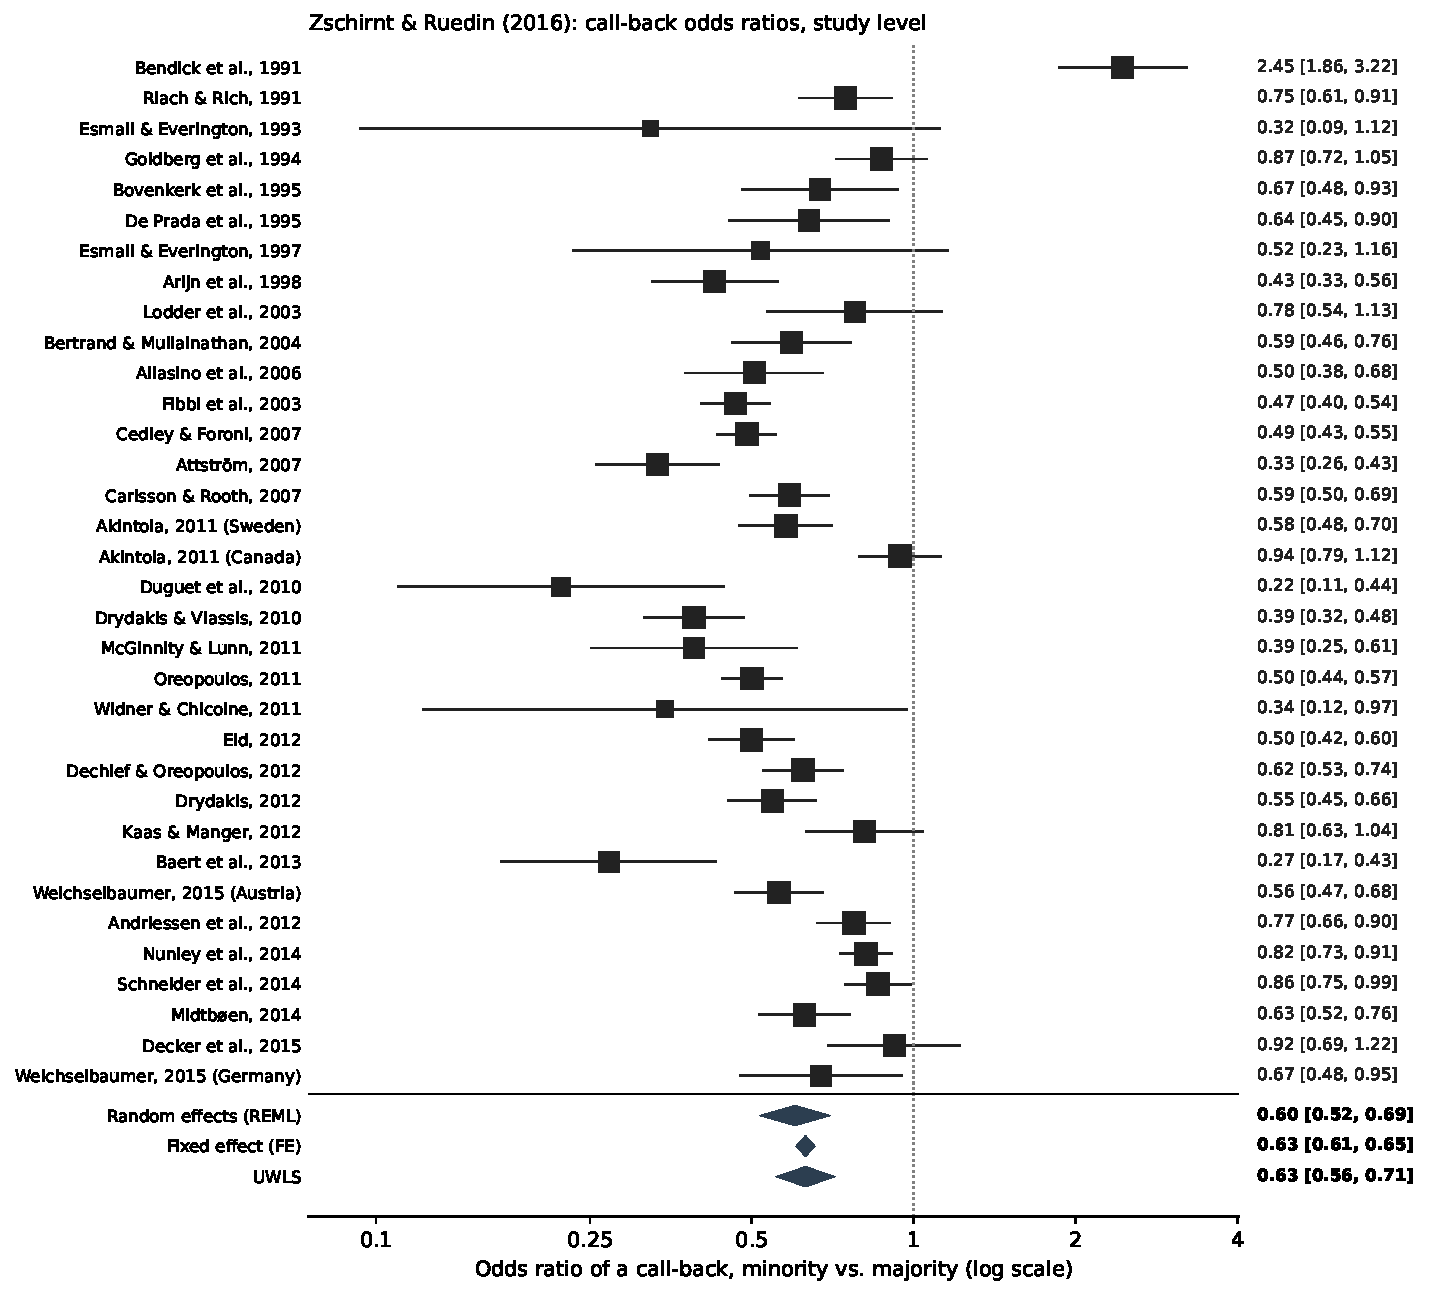
\includegraphics[width=\linewidth]{figures/forest_original.pdf}
  \caption{Forest plot of the original studies}
  \label{fig:forest-original}
\end{figure}

% TODO: FE and UWLS both give \maORfe; the UWLS CI \maCIuwls{} is about
% \maSEratioUWLS{} times wider than the FE CI \maCIfe, because ...

% =====================================================================
\section{Update with new studies}
% both -- task 3
% =====================================================================

\IfFileExists{tables/update_new_studies.tex}{\begin{table}[htbp]
\centering
\small
\caption{New studies compared with the original meta-estimate}
\label{tab:update-new}
\begin{tabular}{llrrrccc}
\toprule
Study & Country & $N$ & OR & 95\% CI & In CI & CIs overlap & In PI \\
\midrule
Koopmans et al., 2019 & Germany & 5'819 & 0.69 & [0.62; 0.78] & no & yes & yes \\
Kline et al., 2022 & US & 83'643 & 0.89 & [0.86; 0.92] & no & no & yes \\
Zschirnt \& Fibbi, 2019 & Switzerland & 1'082 & 0.72 & [0.55; 0.94] & no & yes & yes \\
Adamovic \& Leibbrandt, 2023 & Australia & 12'329 & 0.47 & [0.43; 0.52] & no & no & yes \\
\bottomrule
\end{tabular}
\par\smallskip\parbox{0.95\linewidth}{\footnotesize In CI: OR of the new study lies in the 95\% CI of the original RE estimate [0.52; 0.69]. CIs overlap: the study's own 95\% CI overlaps with it. In PI: lies in the 95\% prediction interval [0.28; 1.27].}
\end{table}
}{}
\IfFileExists{tables/update_pooled.tex}{\begin{table}[htbp]
\centering
\small
\caption{Pooled odds ratio before and after the update}
\label{tab:update-pooled}
\begin{tabular}{lrrr}
\toprule
Method & Original ($k=34$) & With new studies ($k=38$) & Change in OR \\
\midrule
Fixed effect (FE) & 0.63 [0.61; 0.65] & 0.74 [0.72; 0.76] & +17.7\% \\
UWLS & 0.63 [0.56; 0.71] & 0.74 [0.67; 0.81] & +17.7\% \\
Random effects (REML) & 0.60 [0.52; 0.69] & 0.61 [0.54; 0.69] & +1.6\% \\
\bottomrule
\end{tabular}
\end{table}
}{}
\IfFileExists{figures/forest_combined.pdf}{%
\begin{figure}[htbp]
  \centering
  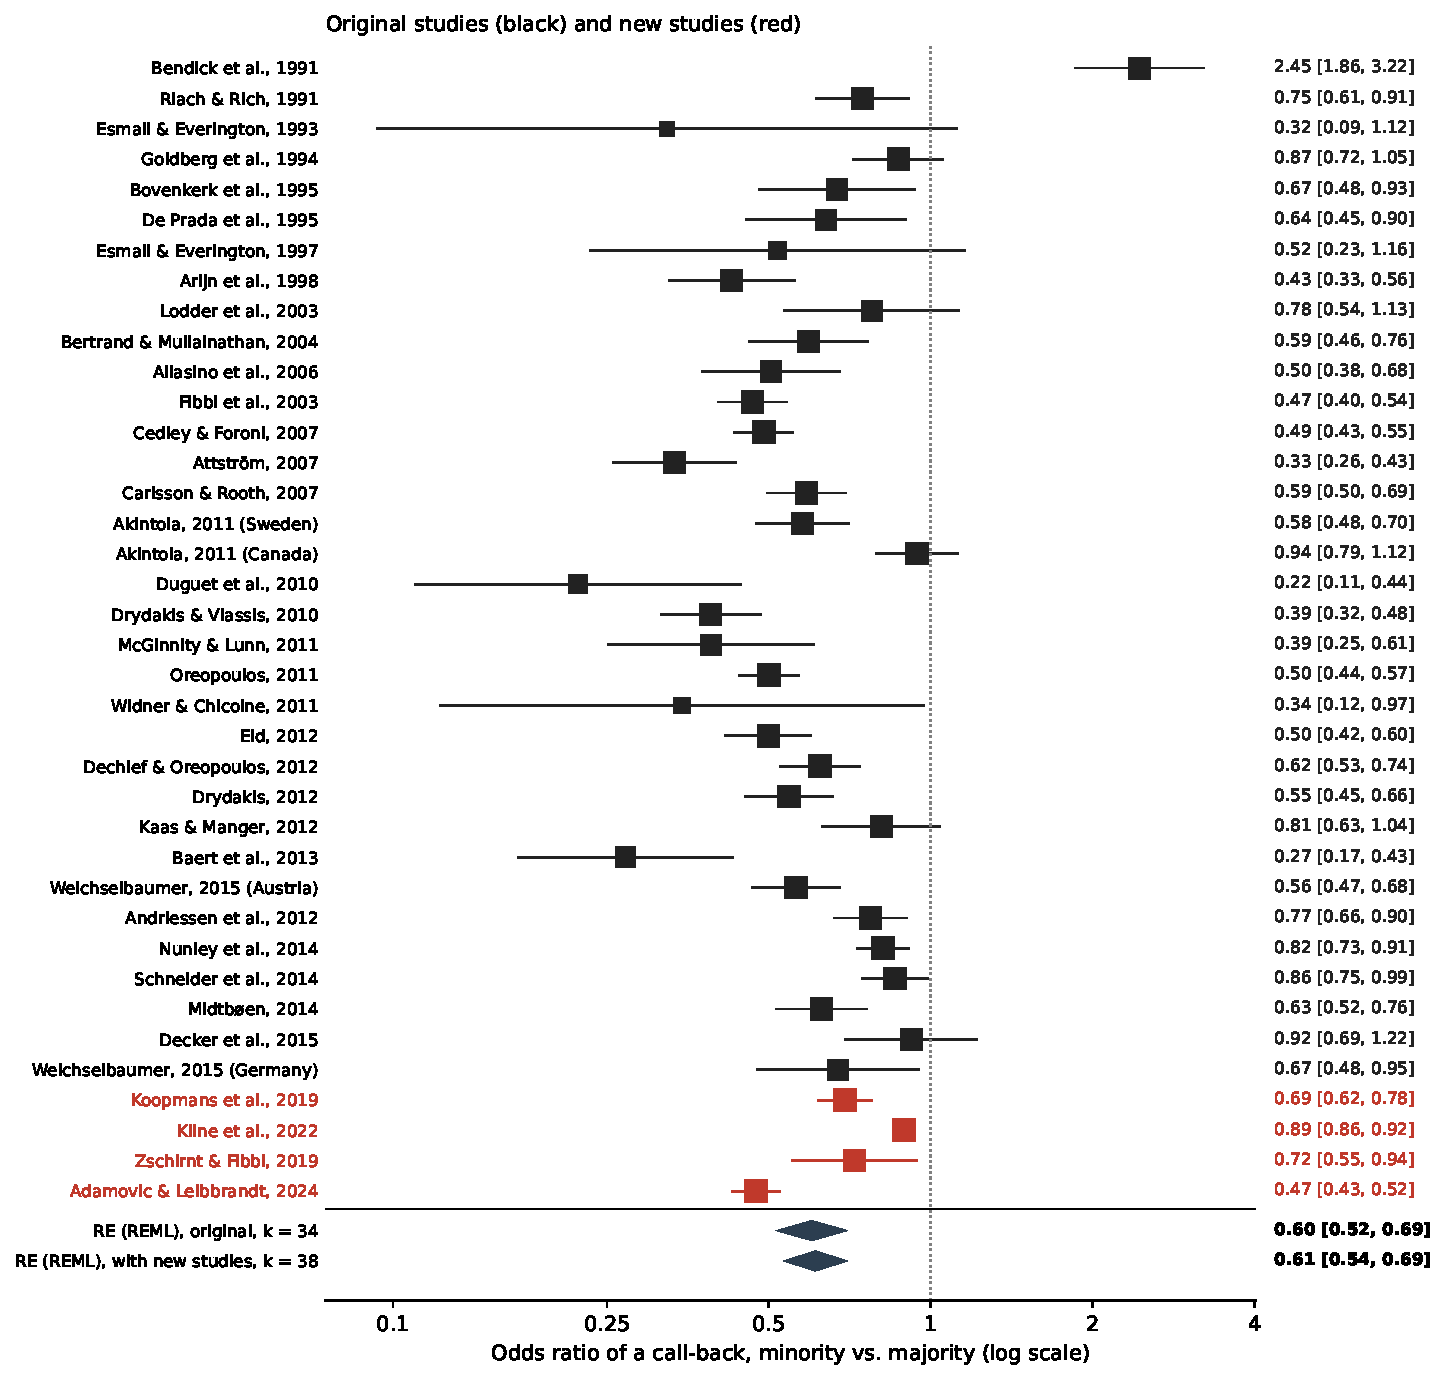
\includegraphics[width=\linewidth]{figures/forest_combined.pdf}
  \caption{Forest plot with the new studies (red)}
  \label{fig:forest-combined}
\end{figure}}{}

% TODO: describe the new studies (\citet{koopmans2019}, \citet{kline2022},
%       \citet{zschirnt2019}, \citet{adamovic2023}); are they inside the CI
%       \maCIre{} and the prediction interval \maPIre? How much does the
%       pooled estimate change?

% =====================================================================
\section{Statistical power}
% both -- task 4
% =====================================================================

\begin{table}[htbp]
\centering
\small
\caption{Statistical power and publication bias}
\label{tab:power-bias}
\begin{tabular}{lrr}
\toprule
 & Original & Original without Bendick (1991) \\
\midrule
$k$ & 34 & 33 \\
Median power & 0.97 & 0.99 \\
Mean power & 0.83 & 0.84 \\
Adequately powered ($q_i \geq 0.8$) & 24 (71\%) & 24 (73\%) \\
FAT: $\hat\beta_1$ (SE) & -1.05 (1.29) & -1.61 (1.09) \\
FAT: $t$ & -0.81 & -1.48 \\
Significant estimates (share) & 27 (0.79) & 26 (0.79) \\
Expected share significant & 0.83 & 0.84 \\
ESS = observed $-$ expected & -0.03 & -0.05 \\
Expected share significant (with $\hat\tau^2$) & 0.70 & 0.73 \\
ESS (with $\hat\tau^2$) & +0.10 & +0.06 \\
\bottomrule
\end{tabular}
\par\smallskip\parbox{0.95\linewidth}{\footnotesize Power of each study at the UWLS estimate: $q_i = \Phi(|\hat\mu|/SE_i - 1.96)$. FAT: slope of the WLS regression of $\ln OR$ on its SE; with discrimination ($\ln OR<0$) selection for significance implies $\beta_1<0$. ESS: observed minus expected share of significant estimates ($|y_i/SE_i|>1.96$); the expected share uses the UWLS estimate as true effect, in the last two rows the true effects vary with $\hat\tau^2$ (REML).}
\end{table}


% TODO: median power \maMedPower; compare with \citet{askarov2024};
%       why is low power a problem, why is our value an upper bound?

% =====================================================================
\section{Publication bias}
% both -- task 5: funnel plot, FAT-PET, WAAP, ESS
% =====================================================================

\begin{figure}[htbp]
  \centering
  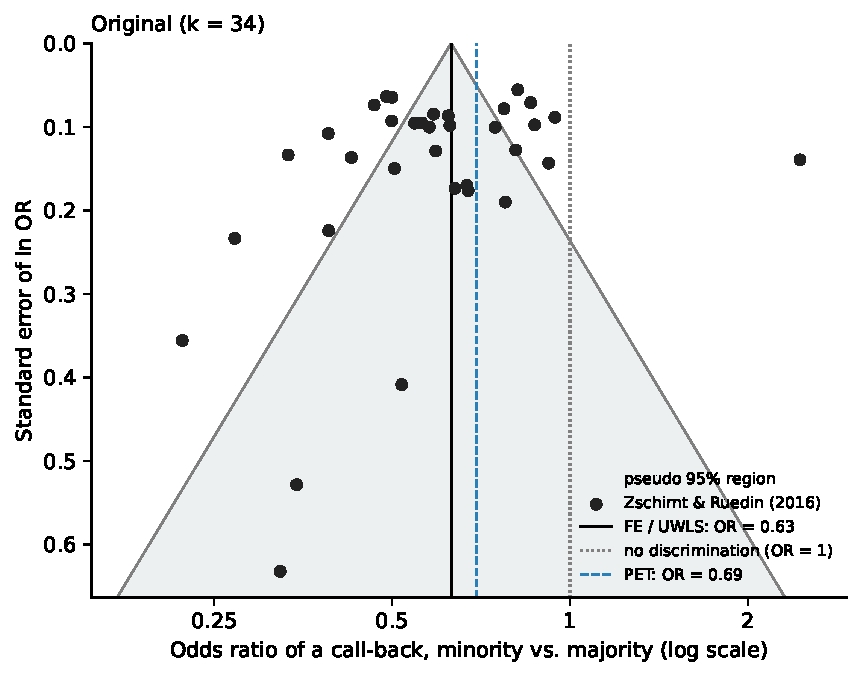
\includegraphics[width=0.75\linewidth]{figures/funnel_original.pdf}
  \caption{Funnel plot of the original studies}
  \label{fig:funnel}
\end{figure}

\begin{table}[htbp]
\centering
\small
\caption{Pooled odds ratios with and without correction for publication bias}
\label{tab:pubbias-estimates}
\begin{tabular}{lrr}
\toprule
Estimator & Original & Original without Bendick (1991) \\
\midrule
Fixed effect (FE) & 0.63 [0.61; 0.65] & 0.62 [0.59; 0.64] \\
UWLS & 0.63 [0.56; 0.71] & 0.62 [0.56; 0.68] \\
Random effects (REML) & 0.60 [0.52; 0.69] & 0.58 [0.52; 0.65] \\
WAAP & 0.64 [0.55; 0.73] & 0.62 [0.55; 0.70] \\
PET & 0.69 [0.53; 0.91] & 0.72 [0.57; 0.90] \\
PEESE & 0.65 [0.57; 0.74] & 0.64 [0.57; 0.71] \\
Adequately powered studies & 24 of 34 & 24 of 33 \\
\bottomrule
\end{tabular}
\par\smallskip\parbox{0.95\linewidth}{\footnotesize OR [95\% CI]. WAAP: UWLS over the studies with power $\geq 80\%$ at the UWLS estimate ($SE_i \leq |\hat\mu_{UWLS}|/2.8$). PET: intercept of the WLS regression $y_i = \beta_0 + \beta_1 SE_i + \varepsilon_i$ (weights $1/SE_i^2$), i.e.\ the effect of a study with $SE \to 0$. PEESE: the same with $SE_i^2$.}
\end{table}


% =====================================================================
\section{Heterogeneity: meta-regression}
% both
% =====================================================================

\begin{table}[htbp]
\centering
\small
\caption{WLS meta-regression: publication bias and heterogeneity (original + new studies)}
\label{tab:metareg-wls}
\begin{tabular}{lrrrrr}
\toprule
 & M1 & M2 & M3 & M4 & M5 \\
\midrule
Intercept (PET) & -0.135** & -0.143** & -0.230 & -0.116 & -0.187 \\
 & (0.061) & (0.059) & (0.197) & (0.174) & (0.138) \\
SE (FAT) & -3.157*** & -1.914* & -0.158 & -2.051 & -1.636 \\
 & (0.861) & (1.039) & (1.371) & (1.336) & (1.319) \\
Europe &  & -0.284** & -0.287* & -0.288** & -0.270* \\
 &  & (0.131) & (0.161) & (0.134) & (0.139) \\
German-speaking country &  & 0.203 & 0.195 & 0.203 & 0.194 \\
 &  & (0.146) & (0.208) & (0.148) & (0.150) \\
High-skilled jobs &  &  & -0.108 &  &  \\
 &  &  & (0.182) &  &  \\
Low-skilled jobs &  &  & -0.172 &  &  \\
 &  &  & (0.155) &  &  \\
Testing year (decades, 0 = 2000) &  &  &  & -0.013 &  \\
 &  &  &  & (0.079) &  \\
New study (update) &  &  &  &  & 0.044 \\
 &  &  &  &  & (0.126) \\
\midrule
$k$ & 38 & 38 & 30 & 38 & 38 \\
Residual SE & 3.54 & 3.41 & 3.16 & 3.46 & 3.46 \\
\bottomrule
\end{tabular}
\par\smallskip\parbox{0.95\linewidth}{\footnotesize WLS with weights $1/SE_i^2$ and multiplicative error (as UWLS), $t$-based standard errors. Dependent variable: $\ln OR$ of a call-back (minority vs.\ majority); negative = discrimination. The intercept is the effect for a study with $SE\to 0$ in the reference group (outside Europe; mixed skills; testing year 2000). * $p<0.1$, ** $p<0.05$, *** $p<0.01$.}
\end{table}


% =====================================================================
\section{Conclusion}
% both -- task 6: is there reliable evidence on the true effect size?
% =====================================================================

% TODO

% =====================================================================
\newpage
\bibliographystyle{apalike}
\bibliography{references}

\appendix
\section{Table of evidence}\label{app:evidence}
{\scriptsize
\setlength{\tabcolsep}{3pt}
\begin{longtable}{>{\raggedright\arraybackslash}p{3.4cm}lr>{\raggedright\arraybackslash}p{3.2cm}rrrr}
\caption{Table of evidence: all studies in the meta-analysis}\label{tab:evidence}\\
\toprule
Study & Country & Test & Minority group & $N$ & CB (\%) & OR [95\% CI] & SE \\
 & & year & & & min. / maj. & & \\
\midrule\endfirsthead
\toprule
Study & Country & Test & Minority group & $N$ & CB (\%) & OR [95\% CI] & SE \\
 & & year & & & min. / maj. & & \\
\midrule\endhead
\bottomrule\endfoot
Bendick et al., 1991 & US & 1991 & Hispanics & 1'482 & 87.6 / 74.2 & 2.45 [1.86; 3.22] & 0.140 \\
Riach \& Rich, 1991 & Australia & 1988 & -- & 1'962 & 25.5 / 31.4 & 0.75 [0.61; 0.91] & 0.101 \\
Esmail \& Everington, 1993 & UK & 1992 & Asian & 46 & 26.1 / 52.2 & 0.32 [0.09; 1.12] & 0.632 \\
Goldberg et al., 1994 & Germany & 1993 & Turkish & 2'786 & 17.5 / 19.6 & 0.87 [0.72; 1.05] & 0.098 \\
Bovenkerk et al., 1995 & Netherlands & 1993 & Surinamese, moroccan & 580 & 35.9 / 45.5 & 0.67 [0.48; 0.93] & 0.170 \\
De Prada et al., 1995 & Spain & 1994 & Moroccan & 538 & 43.5 / 54.6 & 0.64 [0.45; 0.90] & 0.174 \\
Esmail \& Everington, 1997 & UK & 1997 & Asian & 100 & 36.0 / 52.0 & 0.52 [0.23; 1.16] & 0.409 \\
Arijn et al., 1998 & Belgium & 1997 & Moroccans & 898 & 37.4 / 58.4 & 0.43 [0.33; 0.56] & 0.137 \\
Fibbi et al., 2003 & Switzerland & 2002 & -- & 3'276 & 28.5 / 46.1 & 0.47 [0.40; 0.54] & 0.074 \\
Lodder et al., 2003 & US & 2000 & Blacks & 546 & 26.0 / 31.1 & 0.78 [0.54; 1.13] & 0.190 \\
Bertrand \& Mullainathan, 2004 & US & 2001 & African American & 2'646 & 8.2 / 13.2 & 0.59 [0.46; 0.76] & 0.129 \\
Allasino et al., 2006 & Italy & 2005 & Moroccan & 734 & 39.5 / 56.4 & 0.50 [0.38; 0.68] & 0.150 \\
Attström, 2007 & Sweden & 2006 & Native swedes of middle eastern origin & 2'020 & 8.9 / 22.7 & 0.33 [0.26; 0.43] & 0.134 \\
Carlsson \& Rooth, 2007 & Sweden & 2005 & Middle Eastern & 3'104 & 19.7 / 29.4 & 0.59 [0.50; 0.69] & 0.085 \\
Cediey \& Foroni, 2007 & France & 2006 & African & 4'646 & 25.5 / 41.2 & 0.49 [0.43; 0.55] & 0.064 \\
Drydakis \& Vlassis, 2010 & Greece & 2010 & Albanians & 1'578 & 26.1 / 47.5 & 0.39 [0.32; 0.48] & 0.108 \\
Duguet et al., 2010 & France & 2006 & Moroccan & 1'097 & 1.7 / 7.3 & 0.22 [0.11; 0.44] & 0.356 \\
Akintola, 2011 (Sweden) & Sweden & 2009 & Middle eastern/African & 2'018 & 66.2 / 77.2 & 0.58 [0.48; 0.70] & 0.100 \\
Akintola, 2011 (Canada) & Canada & 2009 & Middle eastern & 2'652 & 73.5 / 74.6 & 0.94 [0.79; 1.12] & 0.089 \\
McGinnity \& Lunn, 2011 & Ireland & 2010 & -- & 480 & 15.8 / 32.5 & 0.39 [0.25; 0.61] & 0.224 \\
Oreopoulos, 2011 & Canada & 2008 & English, Indian, Chinese, Pakistani, Chinese with English First name, Greek & 12'910 & 7.6 / 14.2 & 0.50 [0.44; 0.57] & 0.064 \\
Widner \& Chicoine, 2011 & US & 2010 & Arab American & 530 & 1.9 / 5.3 & 0.34 [0.12; 0.97] & 0.528 \\
Andriessen et al., 2012 & Netherlands & 2011 & Moroccans, Turks, Surinamese, Antillians & 2'680 & 39.3 / 45.6 & 0.77 [0.66; 0.90] & 0.078 \\
Dechief \& Oreopoulos, 2012 & Canada & 2010 & English, Indian, Chinese, Chinese with English First name, Greek & 7'991 & 8.3 / 12.7 & 0.62 [0.53; 0.74] & 0.087 \\
Drydakis, 2012 & Greece & 2008 & Albanians & 1'892 & 31.8 / 46.1 & 0.55 [0.45; 0.66] & 0.096 \\
Eid, 2012 & Canada & 2011 & -- & 2'324 & 22.5 / 36.8 & 0.50 [0.42; 0.60] & 0.093 \\
Kaas \& Manger, 2012 & Germany & 2011 & Turkish & 1'056 & 34.7 / 39.6 & 0.81 [0.63; 1.04] & 0.128 \\
Baert et al., 2013 & Belgium & 2011 & Turkish & 673 & 8.0 / 24.2 & 0.27 [0.17; 0.43] & 0.234 \\
Midtbøen, 2014 & Norway & 2013 & Pakistani & 1'800 & 31.9 / 42.8 & 0.63 [0.52; 0.76] & 0.098 \\
Nunley et al., 2014 & US & 2013 & Black & 9'396 & 15.2 / 18.0 & 0.82 [0.73; 0.91] & 0.056 \\
Schneider et al., 2014 & Germany & 2013 & Turkish & 3'376 & 59.9 / 63.5 & 0.86 [0.75; 0.99] & 0.071 \\
Decker et al., 2015 & US & 2011 & Black, hispanics & 3'108 & 7.2 / 7.8 & 0.92 [0.69; 1.22] & 0.143 \\
Weichselbaumer, 2015 (Austria) & Austria & 2012 & Serbian, Turkish, African (Nigeria), Asian (China) & 2'142 & 24.8 / 37.0 & 0.56 [0.47; 0.68] & 0.095 \\
Weichselbaumer, 2015 (Germany) & Germany & 2012 & Turkish & 972 & 13.5 / 18.8 & 0.67 [0.48; 0.95] & 0.176 \\
\end{longtable}
\par\footnotesize $N$: applications sent (minority + majority). CB: call-back rate of minority / majority applicants. OR: odds ratio of a call-back, minority vs.\ majority; SE: standard error of $\ln OR$.
}


\end{document}
